%% grouprank.tex - computing rank with limited nondeterminism
%%
%% Copyright 2014, 2015 Jeffrey Finkelstein.
%%
%% This LaTeX markup document is made available under the terms of the Creative
%% Commons Attribution-ShareAlike 4.0 International License,
%% https://creativecommons.org/licenses/by-sa/4.0/.
\documentclass{article}

\usepackage{amsmath}
\usepackage{amssymb}
%% This must come before hyperref.
\usepackage{amsthm}
%% This is strongly recommended by biblatex.
\usepackage[english]{babel}
\usepackage[backend=biber]{biblatex}
\usepackage[T1]{fontenc}
%% This must come before csquotes.
\usepackage[utf8]{inputenc}
\usepackage{lmodern}
%% This is strongly recommended by biblatex.
\usepackage{csquotes}
%% This must come before hyperref.
\usepackage{thmtools}
%% This must come before complexity.
\usepackage{hyperref}
\usepackage{complexity}
\usepackage[firstpage]{draftwatermark}
\usepackage{mathtools}
\usepackage{microtype}
\usepackage{textcomp}
\usepackage{tikz}

\usetikzlibrary{trees}

\LoadMicrotypeFile{cmr}
\SetProtrusion
    [load=lmr-T1]
    {encoding=T1, family=lmr}
    {
      \textquotedblright = {,1000},
      \textquotedblleft = {1000,},
      {'} = {,1000},
      {,} = {,1000},
      {:} = {,1000},
      {;} = {,1000},
      {.} = {,1000}
    }


%% Set the ``work-in-progress'' watermark for the first page.
\SetWatermarkLightness{0.9}
\SetWatermarkText{Work-in-progress}
\SetWatermarkFontSize{3.5cm}

%% Set the title and author of the PDF file.
\hypersetup{pdftitle={Computing rank of finite algebraic structures with limited nondeterminism}, pdfauthor={Jeffrey Finkelstein}}

%% Declare the bibliography file.
\addbibresource{grouprank.bib}

%% Declare theorem-like environments.
\declaretheorem[numberwithin=section]{theorem}
\declaretheorem[numberlike=theorem,style=definition,qed=\qedsymbol]{example}
\declaretheorem[numberlike=theorem]{lemma}
\declaretheorem[numberlike=theorem]{proposition}
\declaretheorem[numberlike=theorem]{corollary}

%% Custom commands are declared here.
\newcommand{\email}[1]{\textlangle\href{mailto:#1}{\nolinkurl{#1}}\textrangle}
\newcommand{\todo}[1]{\textbf{TODO #1}}
\newcommand{\gen}[1]{\langle #1 \rangle}
\newcommand{\ceil}[1]{\lceil #1 \rceil}
\DeclareMathOperator{\cube}{cube}
\DeclareMathOperator{\rank}{rank}
\DeclareMathOperator{\Path}{Path}
\DeclareMathOperator{\Cay}{Cay}

%% Redefine the footnote environment so it has no reference and no number.
\long\def\symbolfootnote#1{\begingroup%
\def\thefootnote{\fnsymbol{footnote}}\footnotetext{#1}\endgroup}

%% Define the author, title, and date for the document.
\author{Jeffrey~Finkelstein\\ Computer Science Department, Boston University}
\title{Computing rank of finite algebraic structures \\ with limited nondeterminism}
%\date{\today}

\begin{document}

\maketitle

\begin{abstract}
  \begin{abstract}
% Foreword
%
% context (focus on anyone) why now? - current situation, and why the need is so important
The rank of a finite algebraic structure with a single binary operation is the minimum number of elements needed to express every other element under the closure of the operation.
% need (focus on readers) why you? - why this is relevant to the reader, and why something needed to be done
In the case of groups, the previous best algorithm for computing rank used polylogarithmic space.
%%% relevant existing work, given as part of the need
% task (focus on author) why me? - what was undertaken to address the need
We reduce the best upper bounds on the complexity of computing rank for groups and for quasigroups. %%, and provide a theoretically efficient algorithm for the latter.
% object (focus on document) why this document - what the document covers
This paper proves that the rank problem for these algebraic structures can be verified by highly restricted models of computation given only very short certificates of correctness.

% Summary
%
% findings (focus on author) what? - what the work revealed when performing the task
Specifically, we prove that the problem of deciding whether the rank of a finite quasigroup, given as a Cayley table, is smaller than a specified number is decidable by a circuit of depth $O(\log \log n)$ augmented with $O(\log^2 n)$ nondeterministic bits (the complexity class of problems decidable by such circuits is denoted $\bFOLL$).
Furthermore, if the quasigroup is a group, then the problem is also decidable by a Turing machine using $O(\log n)$ space and $O(\log^2 n)$ bits of nondeterminism with the ability to read the nondeterministic bits multiple times (the complexity class for problems like this is denoted $\bL$).
Finally, we provide similar results for related problems on other algebraic structures and other kinds of rank.
% conclusion (focus on readers) so what? - what the findings mean for the audience
These new upper bounds are significant improvements, especially for groups.
% perspective (focus on anyone) what now? - what should be done next
In general, the lens of limited nondeterminism provides an easy way to improve many simple algorithms, like the ones presented here, and we suspect it will be especially useful for other algebraic algorithms.
\end{abstract}

\end{abstract}

\symbolfootnote{%
  Copyright 2014, 2015 Jeffrey~Finkelstein \email{jeffreyf@bu.edu}.

  This document is licensed under the Creative Commons Attribution-ShareAlike 4.0 International License, which is available at \mbox{\url{https://creativecommons.org/licenses/by-sa/4.0/}}.
  The \LaTeX{} markup that generated this document can be downloaded from its website at \mbox{\url{https://github.com/jfinkels/grouprank}}.
  The markup is distributed under the same license.
}

\section{Introduction}
\todo{Rewrite introduction to not have false information.}

% Foreword
%
% context (focus on anyone) why now? - current situation, and why the need is so important
An efficient algorithm computing the rank of a finite algebraic structure (that is, the minimum number of elements required to generate all other elements) benefits mathematicians, who use numerical algebra systems for research, cryptographers, who rely on algebraic systems for proofs of security, and theoretical computer scientists, who seek to understand which problems can be solved in a particular model of computation.
If the structure is, for example, a finite group, then we can represent this structure in one of two reasonable ways.
First, we can represent it as a subset of elements along with a set of equality relations demonstrating how the group operation behaves (known as a group presentation).
Second, we can represent it as a table of values for the binary operation under each pair of input elements (known as a Cayley table or multiplication table).
These representations offer a tradeoff between representation size and the complexity of deciding properties of the group: the latter representation may be exponentially larger than the former, so an efficient algorithm for the latter may not necessarily be efficient for the former.

Consider the situation when the algebraic structure is the finite cyclic group of order $n$.
A natural presentation of this group is $\langle a \, | \, a^n = 1 \rangle$.
Since each element in this group can be represented by $O(\log n)$ bits, the total size of this representation is $O(\log n)$ bits.
In contrast, the Cayley table for this group requires $O(n^2 \log n)$ bits.
Thus, in certain cases, if $m$ represents the size of the input, an algorithm running in time $f(m)$ on inputs of the first form runs in time $O(f(\log m))$ on inputs of the second form.
We can use this to our advantage to construct more efficient algorithms for algebraic problems.

% need (focus on readers) why you? - why this is relevant to the reader, and why something needed to be done
%
%%% relevant existing work, given as part of the need
For quasigroups, the previous best algorithm for computing the rank requires polynomial time in addition to a polylogarithmic amount of nondeterministic bits.
For groups, the previous best algorithm for computing the rank requires a polylogarithmic amount of space, which induces a superpolynomial time (hence, inefficient) algorithm.
Only for certain classes of finite groups was there a polynomial time algorithm.
% task (focus on author) why me? - what was undertaken to address the need
We reduce the best upper bound on the complexity of the rank problem for quasigroups and groups and provide a theoretically efficient algorithm for the latter.
% object (focus on document) why this document - what the document covers
This paper proves that with short certificates of correctness, the rank problem for quasigroups and groups can be verified by highly restricted models of computation, and demonstrates how the same strategy can be applied to semigroups and magmas in general.

% Summary
%
% findings (focus on author) what? - what the work revealed when performing the task
We prove that the problem of deciding whether the rank of a finite quasigroup, given as a Cayley table, is smaller than a specified number is decidable by a circuit of depth $O(\log \log n)$ augmented with $O(\log^2 n)$ nondeterministic bits (the complexity class of problems decidable by such circuits is denoted $\bFOLL$).
Furthermore, if the quasigroup is a group, then the problem is also decidable by a Turing machine using $O(\log n)$ space and $O(\log^2 n)$ bits of nondeterminism (the complexity class for problems like this is denoted $\bL$).
The general strategy is to reduce the problem of computing rank to the problem of computing membership; we compute the rank of a group by guessing a small set of candidate generators, then deciding whether each other element in the group can be generated from that set.
For the sake of completeness, we show how this strategy applies to semigroups and magmas in general, though the results are less interesting there because these algebraic structures lack two things that the groups and quasigroups have: small generating sets and efficient membership algorithms.
The problem is in $\NL$ for semigroups and in $\NP$ for general magmas.
Finally, we show that the problem for rings is in $\NL$ as well.
\autoref{tab:summary} summarizes these improvements, and \autoref{fig:inclusions} demonstrates graphically why these improvements are so significant.
(We could not find an explicit upper bound for magmas and semigroups, but other papers imply that the problems are in $\NP$.)
\begin{table}
  \caption{\label{tab:summary}We improve algorithms for computing rank of finite algebraic structures.}
  \begin{center}
    \begin{tabular}{r l l}
      & old & new \\[5pt]
      magma & $\NP$ & $\NP$ \\
      semigroup & $\NP$ & $\NP$ \\
      quasigroup & $\bP$ \autocite{py96} & $\bFOLL$ \\
      group & $\L^2$ \autocite{lsz77} & $\bFOLL \cap \bL$ \\
      ring & $\NP$ & $\NL$
    \end{tabular}
  \end{center}
\end{table}
\begin{figure}
  \caption{\label{fig:inclusions}Hierarchies of complexity classes with limited nondeterminism can circumvent common deterministic complexity classes.}
  \begin{center}
    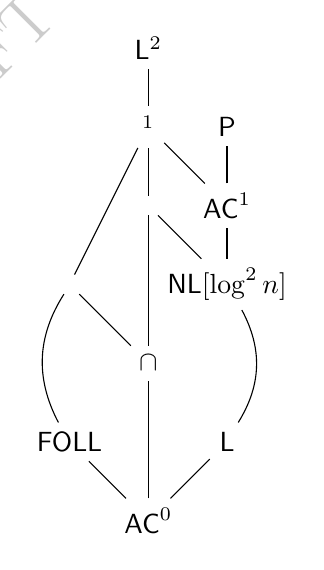
\begin{tikzpicture}
      \node at ( 0, 6) (l2) {$\L^2$};
      \node at ( 1, 5) (p) {$\P$};
      \node at ( 0, 5) (bac1) {$\bAC^1$};
      \node at ( 1, 4) (ac1) {$\AC^1$};
      \node at ( 0, 4) (bl) {$\bL$};
      \node at ( 1, 3) (nllog2) {$\NL[\log^2 n]$};
      \node at (-1, 3) (bfoll) {$\bFOLL$};
      \node at ( 0, 2) (bfollandbl) {$\bFOLL \cap \bL$};
      \node at (-1, 1) (foll) {$\FOLL$};
      \node at ( 1, 1) (l) {$\L$};
      \node at ( 0, 0) (ac0) {$\AC^0$};
      \draw (ac0) to (l);
      \draw (ac0) to (foll);
      \draw (ac0) to (bfollandbl);
      \draw[bend left] (foll) to (bfoll);
      \draw[bend right] (l) to (nllog2);
      \draw (nllog2) to (bl);
      \draw (bfollandbl) to (bl);
      \draw (bfollandbl) to (bfoll);
      \draw (bfoll) to (bac1);
      \draw (bl) to (bac1);
      \draw (nllog2) to (ac1);
      \draw (ac1) to (bac1);
      \draw (ac1) to (p);
      \draw (bac1) to (l2);
    \end{tikzpicture}
  \end{center}
\end{figure}

% conclusion (focus on readers) so what? - what the findings mean for the audience
These are improvements on the previous best upper bounds for these problems.
Previously, the best upper bound for computing the rank of a quasigroup given as a Cayley table was $\bP$ \autocite[Section~5]{py96} and for groups, $\L^2$ \autocite{lsz77} (see also \cite[Proposition~6]{at06} for a brief description of the algorithm).
Our results are an improvement because
\begin{equation*}
  (\bFOLL \cap \bL) \subseteq \NL \subseteq (\L^2 \cap \P).
\end{equation*}
%% This is an improvement because
%% \begin{align*}
%%   (\bFOLL \cap \bL) & \subseteq \bL \subseteq \NL \subseteq \AC^1 \subseteq \bAC^1, \\ %\subseteq \bNC^2 \subseteq \L^2,
%%   (\bFOLL \cap \bL) & \subseteq \bFOLL \subseteq \bAC^1, %\subseteq \bNC^2 \subseteq \L^2.
%% \end{align*}
%% and
%% $$
%% \bAC^1 \subseteq \bNC^2 \subseteq \L^2.
%% $$
%% (In the last inclusion we use the fact that $\bNC^2 \subseteq \L^2$ \cite[Lemma~3.1]{wolf94}.)
This also improves the result of \cite[Theorem~7]{at06}, which shows that computing the rank of a nilpotent group is in $\P$.
However, the relationship between $\FOLL$ and $\L$ remains unknown (the best inclusion known is the uninteresting inclusion $\FOLL \subseteq \AC^1$), so the relationship between $\bFOLL$ and $\bL$ is unknown as well.
Still, for groups, the problem is decidable by an extremely restrictive computational model, and so can be simulated by a deterministic Turing machine in polynomial time.
Finally, contrast the complexity of the rank problem for groups with the complexity of computing the rank of a subgroup of a free group.
The latter problem is $\P$-complete, so is not even in $\NC$ unless $\NC = \P$ \autocite[Theorem~4.9]{am84} (see also \autocite[Problem~A.8.11]{ghr95}).

% perspective (focus on anyone) what now? - what should be done next

Using limited nondeterminism and restrictive models of computation as verifiers may also be useful in examining other problems.
The limited nondeterminism lens specifically suggests some opportunities for further research in computational algebra, though it has seen some recent success in other subfields of theoretical computer science (see \autocite{gottlob13}, for example).
Here are some avenues for future research.
\begin{itemize}
\item Is computing the rank of a quasigroup also in $\bL$?
\item
  Is the group rank problem in a smaller complexity class, one contained in both $\bFOLL$ and $\bL$?
  What is the largest complexity class we can find that is in $\FOLL \cap \L$?
  This would likely improve all the results in \autocite{bklm01}.
\item Is there a reduction between the problem of computing the rank of a quasigroup and the problem of deciding whether two quasigroups are isomorphic?
\item Is the problem of computing the shortest generating sequence for a quasigroup strictly more difficult than the problem of computing the rank of a quasigroup?
\item
  The complexity of group problems, for example, varies based on the succinctness of the representation of the input.
  In this paper we show that the rank problem is quite easy when the input is given its least succinct representation, the full Cayley table.
  On the other hand, in the most succinct representation, the group presentation (a set of generators for the group along with relations among the generators), many problems become very difficult, or even undecidable if the group is infinite.
  For representations of intermediate succinctness, for example a circuit that outputs the entries of the Cayley table, how difficult is the rank problem?
\end{itemize}


\section{Preliminaries}

Here, $\log n$ denotes the base two logarithm of $n$, for any natural number $n$.
Also, the set $\{1, \dotsc, n\}$ is denoted $[n]$.

\subsection{Complexity}

Here is a brief summary of the definitions of the complexity classes that appear in this paper.

\begin{itemize}
\item
  $\L$ is the class of languages decidable by a deterministic Turing machine that uses $O(\log n)$ space on inputs of length $n$.
  $\L^2$ is similar, but with $O(\log^2 n)$ space.
\item
  $\NL$ is the class of languages decidable by a nondeterministic Turing machine that uses $O(\log n)$ space.
  Equivalently, this is the class of languages $L$ for which there is a deterministic Turing machine with a two-way read-only tape for the input string, a one-way read-only tape for the nondeterministic bits, and a two-way read-write work tape in which only $O(\log n)$ cells are used, such that $x \in L$ if and only if there is a binary string $w$ of polynomial length such that the machine accepts on input $x$ and nondeterministic bits $w$.
\item $\NL[\log^2 n]$ is the subclass of $\NL$ in which the length of $w$ is bounded by $O(\log^2 n)$.
\item $\bL$ is the superclass of $\NL[\log^2 n]$ in which the machine has two-way access to the tape containing the nondeterministic bits.
  Equivalently, this is the class of languages $L$ such that there is a language $L' \in L$ such that $x \in L$ if and only if there is a binary string $w$ of length $O(\log^2 n)$ such that $(x, w) \in L'$.
\item
  $\FOLL$ is the class of languages decidable by a $\L$-uniform family of circuits with polynomial size, unbounded fan-in, and $O(\log \log n)$ depth.
  $\bFOLL$ is the class of languages decidable by $\FOLL$ circuits that have been augmented with $O(\log^2 n)$ nondeterministic bits (gates with no inputs and one output).
\item
  $\AC^0$ and $\bAC^0$ are the restrictions of $\FOLL$ and $\bFOLL$, respectively, to depth $O(1)$.
  $\NAC^0$ allows a polynomial number of nondeterministic bits.
\end{itemize}
In general, the class $\beta_2 \mathcal{C}$ is the class of languages decidable by $\mathcal{C}$ machines augmented with $O(\log^2 n)$ bits of nondeterminism, or equivalently, the class of languages verifiable by $\mathcal{C}$ machines when given a certificate of length $O(\log^2 n)$.

If $L_1$ and $L_2$ are languages, there is a \emph{logarithmic space many-one reduction} from $L_1$ to $L_2$, denoted $L_1 \leq_m^{\L} L_2$, if there is a function $f$ such that $f$ is computable in logarithmic space and $x \in L_1$ if and only if $f(x) \in L_2$.
%%\todo{CORRECT THIS DEFINITION to be more clear about nondeterministic function outputs (exists/forall)}
%% SHOWS UP IN A LATER SECTION \todo{Does Immerman-Szelpcsenyi Theorem apply to $\bL$?}
%% NO It seems not, since it would require guessing up to m shortcut edges. \todo{Is directed planar graph reachability in $\beta \L$? In $\NL[\log^{O(1)} n]$? See ``shortcut graphs'' by Thorup.}
\todo{Explain why the closure of L under beta AC reductions is probably not NL[log2 n], and maybe prove it?.}
There is a \emph{$\bAC^0$ conjunctive truth-table reduction} from $L_1$ to $L_2$, denoted $L_1 \leq^{\bAC^0}_{ctt} L_2$, if there is a function $f$ and a polynomial $p$ such that
\begin{itemize}
\item $f$ is computable in $\AC^0$,
\item $x \in L_1$ if and only if there is a $w$ of length $O(\log^2 n)$ such that $\bigwedge_{i = 1}^{p(n)} y_i \in L_2$, where $f(x, w) = (y_1, \dotsc, y_{p(n)})$.
\end{itemize}
A $\NAC^0$ conjunctive truth-table reduction is the generalization in which $f$ receives a witness of length polynomial in $n$, instead of polylogarithmic in $n$.
A reduction of this form is really a nondeterministic polynomial-time conjunctive truth-table reduction, since $\NAC^0 = \NP$.

\begin{lemma}\label{lem:ctt}
  Suppose $L_1$ and $L_2$ are languages.
  \begin{enumerate}
  \item If $L_1 \leq^{\NAC^0}_{ctt} L_2$ and $L_2$ is in $\P$, then $L_1$ is in $\NP$.
  %% THIS IS FALSE, nondeterministic functions don't compose: \item If $L_1 \leq^{\NAC^0}_{ctt} L_2$ and $L_2$ is in $\NL$, then $L_1$ is in $\NL$.
  \item If $L_1 \leq^{\bAC^0}_{ctt} L_2$ and $L_2$ is in $\FOLL$, then $L_1$ is in $\bFOLL$.
  \item If $L_1 \leq^{\bAC^0}_{ctt} L_2$ and $L_2$ is in $\L$, then $L_1$ is in $\bL$.
  \end{enumerate}
\end{lemma}
\begin{proof}
  In each case, let $f$ denote the reduction, $M_2$ denote the machine that decides $L_2$, and $q(n)$ denote the polynomial that bounds the number of outputs produced by $f$.
  We construct a nondeterministic machine $M_1$ of the appropriate type as follows on input $x$ of length $n$.
  Nondeterministically choose a string $w$ of the appropriate length (polynomial or polylogarithmic), simulate $f(x, w)$, then run $M_2$ on each $y_i$, where $f(x, w) = (y_1, \dotsc, y_{q(n)})$.
  The machine $M_1$ accepts if and only if each of the simulations of $M_2$ accepts.
  The correctness of $M_1$ follows from the correctness of $f$ and $M_2$.
  The only remaining issue is the complexity of $M_1$.

  In the first case, the $\NP$ machine $M_1$, after choosing its nondeterministic bits, can simulate $f$ in polynomial time and can simulate a polynomial number of instances of $M_2$ in polynomial time.

  For the last two cases, we use the fact that $\bAC^0 \subseteq (\bFOLL \cap \bL)$.
  If $L_2$ is in $\FOLL$, we define $M_1$ to be the circuit
  \begin{equation*}
    M_1(x, w) = \bigwedge_{i = 1}^{q(n)} M_2(y_i),
  \end{equation*}
  where $n$ is the length of $x$, the string $w$ is the nondeterministic string of length $O(\log^2 n)$, and $q(n)$ is the polynomial bounding the number of outputs of $f$ on inputs of length $n$.
  The depth of the $M_1$ circuit is the depth of $f$ plus the depth of $M_2$, which is $O(1) + O(\log \log n)$, or simply $O(\log \log n)$.
  The number of nondeterministic bits required by $M_1$ is the same as the number of nondeterministic bits required by $f$, which is $O(\log^2 n)$.
  The circuit is polynomial in size because $f$ is polynomial in size, $M_2$ is polynomial in size, and there are a polynomial number of parallel instances of the circuit $M_2$.
  Thus $M_1$ is in $\bFOLL$.

  The proof is similar if $L_2$ is in $\L$.
  The only difference is that instead of a circuit computing the conjunction of $q(n)$ bits, we loop over each $y_i$ and check if each one causes $M_2$ to accept.
  Since there are a polynomial number of them, indexing them requires only logarithmic space.
  We also require the fact that logarithmic space computable functions compose.
\end{proof}

Conondeterministic reductions yield similar closures.

Finally, if $L$ is a language and $F$ is a function, there is a \emph{nonadaptive $\AC^0$ Turing reduction} from $L$ to $F$ if there is an $\AC^0$ function $g$ and an $\AC^0$ circuit $C$ such that $x \in L$ if and only if $C(x, F(y_1), \dotsc, F(y_m)) = 1$, where $(y_1, \dotsc, y_m)$ is the output of $g(x)$ and $m$ is bounded by a polynomial in $|x|$.
The function $g$ is called the \emph{generator of the reduction} and the circuit $C$ is called the \emph{evaluator of the reduction}.

\subsection{Algebra}

A \emph{magma} is a set $G$ with a binary operation $\cdot$ that is closed on $G$.
Unless otherwise stated, we will only consider \emph{finite magmas}, in which $G$ is a finite set.
The \emph{Cayley table} of a magma with $n$ elements is the $n \times n$ table whose rows and columns are indexed by the elements of $G$ and where entry $(a, b)$ has value $c$ if $a \cdot b = c$.
If the binary operation is associative, the magma is called a \emph{semigroup}.
A semigroup with a unique identity element is called a \emph{monoid}.
If the binary operation has the property that for each $a$ and $b$ in $G$ there are unique elements $x$ and $y$ in $G$ such that $a \cdot x = b$ and $y \cdot a = b$, the magma is called a \emph{quasigroup}.
(In other words, each quasigroup element appears exactly once in each row and each column of the Cayley table of $G$, or the Cayley table is a \emph{Latin square}.)
If a quasigroup is nonempty and associative, then it is a \emph{group}.
Alternately, if a semigroup has an identity and inverses, then it is a group.
%% Thus if a magma is nonempty, a semigroup, and a quasigroup, it is a group.

\begin{example}\label{ex:quasigroup}
  The smallest nonempty quasigroup that is not also a group has three elements, $\{a, b, c\}$.
  Its Cayley table is
  \begin{equation*}
    \begin{array}{c | c c c}
      \cdot & a & b & c \\
      \hline
      a & a & b & c \\
      b & c & a & b \\
      c & b & c & a \\
    \end{array}
  \end{equation*}
  Examining the table reveals that there is exactly one of each quasigroup element in each row and column.
  This quasigroup is not associative because $b \cdot (a \cdot b) = b \cdot b = a$ but $(b \cdot a) \cdot b = c \cdot b = c$.
  Also, it has a left identity, $a$, but no right identity.
\end{example}

\begin{example}\label{ex:zero}
  The \emph{right zero semigroup} is the semigroup in which each element is a right zero.
  Its Cayley table is
  \begin{equation*}
    \begin{array}{c | c c c}
      \cdot & a & b & c \\
      \hline
      a & a & b & c \\
      b & a & b & c \\
      c & a & b & c \\
    \end{array}
  \end{equation*}
  The associativity of this semigroup can be determined by examining all possible triples $(x, y, z)$ in $G^3$ and checking that $(x \cdot y) \cdot z = x \cdot (y \cdot z)$.
  Each element of this semigroup is a left identity and a right zero, but there are no right identities, so it is not a group.

  Unlike for the Latin square property in the previous example, there is no obvious way to tell whether a binary operation is associative simply by scanning the rows and columns.
  In other words, given only its Cayley table, determining whether a magma is a quasigroup \emph{seems} easier than determining whether a magma is a semigroup.
  However, there is a polynomial time algorithm, attributed to F.~W.~Light, for deciding whether a magma is associative; it is simply the naïve algorithmic implementation of the associativity condition.
\end{example}

\begin{example}
  There is a unique (up to isomorphism) group on three elements $\{a, b, c\}$.
  Its Cayley table is
  \begin{equation*}
    \begin{array}{c | c c c}
      \cdot & a & b & c \\
      \hline
      a & a & b & c \\
      b & b & c & a \\
      c & c & a & b \\
    \end{array}
  \end{equation*}
  This group is the group of integers under addition modulo three.
  It is both a semigroup and a quasigroup.
\end{example}

A \emph{parenthesization} $P$ of a sequence of magma elements $(g_1, \dotsc, g_k)$ is a binary tree that has the magma elements as its leaves (in the order indicated by the sequence).
The \emph{parenthesized product} of a sequence of magma elements $(g_1, \dotsc, g_k)$ with parenthesization $P$, denoted $P(g_1, \dotsc, g_k)$, is the element that results from performing the magma operation in the order indicated by the parenthesization.

\begin{example}
  Consider $(a, c, a, b)$, a sequence of four elements from the quasigroup defined in \autoref{ex:quasigroup}.
  One parenthesization of this sequence is
  \begin{equation*}
    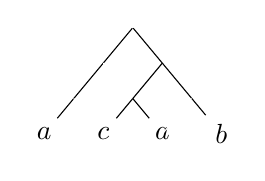
\begin{tikzpicture}[xscale=0.5, yscale=0.3]
      \node[minimum size=0pt, inner sep=0pt] {}
      child {
        child {
          child {node {$a$}}
          child[color=white] {}
        }
        child[color=white] {}
      }
      child {
        child {
          child {node {$c$}}
          child {node {$a$}}
        }
        child {
          child[color=white] {}
          child {node {$b$}}
        }
      };
    \end{tikzpicture}
  \end{equation*}
  which corresponds to the parenthesized product $a \cdot ((c \cdot a) \cdot b)$.
  According to the Cayley table, this product equals $a$.
\end{example}

\begin{lemma}\label{lem:product}
  For any quasigroup on $n$ elements given as a Cayley table, any sequence $(g_0, \dotsc, g_k)$, and any parenthesization $P$ of depth $d$ on that sequence, the parenthesized product $P(g_0, \dotsc, g_k)$ can be computed by an $\L$-uniform family of unbounded fan-in circuits with size $O(k n^2 \log n)$ and depth $O(d)$.
\end{lemma}
\begin{proof}
  How does a circuit access and use a Cayley table for a quasigroup?%
  \footnote{We avoid representing problems using first-order logic, as in the original definition of $\FOLL$ from \autocite{bklm01}, though the logic definition may provide a more natural representation of this sort of information.}
  One way for a circuit to compute the product of two quasigroup elements using the Cayley table is via a multiplexer.
  In the multiplexer, each input has $O(\log n)$ bits, since each quasigroup element can be represented with $O(\log n)$ bits and each input is a pair of quasigroup elements.
  A multiplexer that selects from $n^2$ inputs, each of length $O(\log n)$, can be implemented by an \emph{unbounded fan-in} circuit of depth $O(1)$ and size $O(n^2 \log n)$.
\end{proof}

If $S$ is a subset of magma elements, the \emph{submagma} generated by $S$, denoted $\gen{S}$, is the closure of $S$ under the magma operation and under any parenthesization.
(For semigroups, and hence for groups, the operation is associative, so the parenthesization is superfluous.)
If $\gen{S} = G$, then $S$ is called a \emph{generating set for $G$}.
The \emph{rank of a magma $G$}, denoted $\rank(G)$, is the minimum cardinality of a generating set.
This terminology extends to semigroups and groups as well.

\begin{example}\label{ex:semigroupgen}
  Consider the right zero semigroup on $n$ elements, a generalization of \autoref{ex:zero}.
  In this semigroup, call it $G$, we have $x \cdot y = y$ for each $x$ and $y$ in $G$.
  The rank of this semigroup must be $n$.
  Assume for the sake of producing a contradiction that the rank is strictly less than $n$.
  Thus there is an element $z$ not in the generating set such that $x_1 \cdot \dotsb \cdot x_n = z$, where each $x_i$ is an element of the generating set.
  This is a contradiction with the fact that $x_1 \cdot \dotsb \cdot x_n = x_n$, since $x_n$ is a right zero.
  Therefore the rank of the semigroup must be $n$.
\end{example}

\begin{example}\label{ex:elementary}
  Consider the elementary abelian $2$-group, $(\mathbb{Z} / 2 \mathbb{Z})^k$, for some positive integer $k$.
  Let $n$ denote the order of this group, so $n = 2^k$.
  The minimum generating set for this group is $\{e_1, \dotsc, e_k\}$, where $e_i$ is the $k$-tuple with a one in the $i$th position and a zero in each other position (if we consider the group as a vector space, $e_i$ is the standard basis vector).
  Thus the group has a minimum generating set of size $k$, which is $\log n$.
\end{example}

For quasigroups, we consider a slightly more specific notion of ``generating''\kern-0.5em.
If $(g_0, \dotsc, g_k)$ is a finite sequence of quasigroup elements denoted $S$ and $P$ is a parenthesization of that sequence, then the \emph{cube of $S$ with respect to $P$}, denoted $\cube_P(S)$, is defined
\begin{equation*}
  \cube_P(S) = \left\{P(g_0, g_1^{\epsilon_1}, \dotsc, g_k^{\epsilon_k}) \, \middle| \, \epsilon_i \in \{0, 1\} \text{ for each } i \right\},
\end{equation*}
where $g_i^{\epsilon_i}$ denotes $g_i$ if $\epsilon_i = 1$ and the empty word if $\epsilon_i = 0$.
The element $g_0$ has no exponent because the empty word by itself is not an element in a quasigroup.
(This is called a ``cube'' because each vertex of the $k$-dimensional Boolean hypercube, when interpreted as a binary string $\epsilon_1 \dotsb \epsilon_k$, yields a quasigroup element.)
If $\cube_P(S) = G$, then $g$ is called a \emph{cube generating sequence of size $k + 1$} for the quasigroup $G$.
The \emph{rank of a quasigroup $G$}, denoted $\rank(G)$, is the minimum size of a cube generating sequence.%
\footnote{
  This is a nonstandard definition of ``rank'' for quasigroups.
  Elsewhere, the rank of a quasigroup is the number of blocks in the partition of the quasigroup into conjugacy classes according to the action of the quasigroup on itself.
}
Contrast the rank of a quasigroup with the rank of a semigroup: the former is the size of a sequence, the latter the size of a set.

%% \begin{example}
%%   \todo{Example of a cube generating sequence for a quasigroup.}
%% \end{example}

Ideally, we would like the notion of rank to be identical for each algebraic structure.
If a quasigroup has a cube generating sequence of size at most $k$, then it has a generating set of size at most $k$, specifically the set of distinct elements from the sequence.
However, we conjecture that for sufficiently large sizes, there is a quasigroup that has a generating set of size strictly less than the size of its minimum cube generating sequence.
If this is incorrect, that is if a small generating set implies a small cube generating sequence, we could use the same definition of rank for all our algebraic structures, simplifying our proofs.

Quasigroups have small cube generating sequences, and groups have small generating sets.
As of this publication, upper bounds on the size of generating sets for semigroups remain the subject of research \autocite{gray14}, although in general, some semigroups of order $n$ have rank $n$ (see \autoref{ex:semigroupgen}).
Magmas have even less structure than semigroups, and hence lack a meaningful upper bound as well.

An upper bound for the minimum size of a generating set for quasigroups can be proven by the probabilistic method.

\begin{lemma}[{\autocite[Theorem~3.3]{ctw13}}]\label{lem:small}
  Each finite quasigroup with $n$ elements has a cube generating sequence of size $O(\log n)$ with a parenthesization of depth $O(\log \log n)$.
\end{lemma}

Since a group is a quasigroup, and since a cube generating sequence induces a generating set, the same upper bound can be applied to groups.
However, a more specific (and constructive) upper bound can be proven inductively by considering cosets of increasing size.

\begin{lemma}\label{lem:log}
  If $G$ is a finite group of order $n$ then the minimum size of a generating set is at most $\log n$, with equality when the group is a finite elementary abelian $2$-group.
\end{lemma}
\begin{proof}[Proof (expanded from \autocite{arvind07})]
  %This proof is an expanded version of the proof from \autocite{arvind07}.
  %
  Suppose $m$ is the size of the minimum generating set.
  Let $H_0 = \gen{e}$, where $e$ is the identity element in $G$.
  For each $i \in [m]$, let $H_i = \gen{H_{i - 1} \cup \{x_i\}}$ where $x_i \in G \setminus H_{i - 1}$.
  Such an $x_i$ must exist for each $i$ because otherwise we would have some set $H_j$, of size less than $m$, which generates the group $G$; this violates the hypothesis that $m$ is the minimum size of a generating set for $G$.

  Now, for each $i \in [m]$, we have $x_i \neq e$, by construction.
  Furthermore, the cosets $x_i \gen{H_{i - 1}}$ and $e \gen{H_{i - 1}}$ are disjoint.
  If we suppose to the contrary that there is some element $y \in e \gen{H_{i - 1}} \cap x_i \gen{H_{i - 1}}$, then $y = x_i h$ for some $h \in H_{i - 1}$, which implies $x_i = yh^{-1}$, and hence $x_i \in H_{i - 1}$ since both $y$ and $h$ are in $H_{i - 1}$.
  This is a contradiction with the hypothesis that $x_i \in (G \setminus H_{i - 1})$.
  Therefore $|H_i| \geq 2 |H_{i - 1}|$.
  By induction, $|G| = |H_m| \geq 2^m$, which implies $m \leq \log |G| = \log n$.

  The equality follows from \autoref{ex:elementary}.
\end{proof}
%% \todo{Are there subclasses of semigroups that have logarithmic size generating sets, possibly by a non-constructive existential proof via the probablistic method?
%%   For semigroups, it seems the rank can be computed from the complicated formulas in \autocite{gray14}.}

\begin{example}
  This lemma is particularly interesting to me with respect to the following example.
  \todo{This note doesn't particularly belong here, it should be removed; it's just here so I remember it.}

  Let $G$ and $H$ be finite groups of order $m$ and $n$, respectively.
  Let $S$ and $T$ be generating sets for $G$ and $H$, respectively.
  By the previous lemma, $|S| \leq \log m$ and $|T| \leq \log n$.
  Since $S$ and $T$ are generatings sets, $S \times T$ is a generating set for $G \times H$.
  But $|S \times T| = |S| |T| \leq (\log m) (\log n)$, whereas $\log |G \times H| = \log |G| |H| = \log |G| + \log |H| = \log m + \log n$.
  Thus $G \times H$ has a generating set strictly smaller than $S \times T$, for sufficiently large $m$ and $n$.

  This is surprising to me because I would expect the direct product of $G$ and $H$ to behave like the span of two independent spaces.
  In graph terms, let $\Cay(G, S)$ and $\Cay(H, T)$ be the Cayley graphs of $G$ and $H$ with edges labeled by elements of $S$ and $T$, respectively.
  According to \autocite[Proposition~7]{heydemann97},
  \begin{equation*}
    \Cay(G \times H, S \times T) = \Cay(G, S) \times \Cay(H, T),
  \end{equation*}
  where the first $\times$ is the direct product of groups, the second is the Cartesian product of sets, and the third is the tensor product of labeled graphs.
  A step in a tensor product graph is like two independent steps in the factor graphs.
\end{example}

\section{Computation of submagma membership}
% Foreword
%
% context (focus on anyone) why now? - current situation, and why the need is so important
As stated in the introduction, computing the rank of a magma reduces to the problem of deciding submagma membership.
% need (focus on readers) why you? - why this is relevant to the reader, and why something needed to be done
Thus, in order to determine an upper bound on the complexity of computing the rank, we can determine the complexity of deciding membership.
%
%%% relevant existing work, given as part of the need
Fortunately, the membership problem for a submagma when the magma is given as its Cayley table is a well-studied problem.
% task (focus on author) why me? - what was undertaken to address the need
% object (focus on document) why this document - what the document covers
This section reviews the complexity for the membership problem for magmas, semigroups, quasigroups, and groups.

% Summary
%
% findings (focus on author) what? - what the work revealed when performing the task
We recall that for magmas the membership problem, given the Cayley table, is in $\NP$ and for semigroups $\NL$.
We prove that for quasigroups the problem is in $\FOLL$ and for groups $\L$.
% conclusion (focus on readers) so what? - what the findings mean for the audience
These upper bounds allow us to prove upper bounds on the rank problem in the next section.
% perspective (focus on anyone) what now? - what should be done next
If future work reveals more efficient algorithms for the membership problem for quasigroups or groups, we can provide improved algorithms for computing the rank of these algebraic structures.

The \textsc{Submagma Membership} problem is defined as follows.
The inputs are a magma $G$ given as a Cayley table, a magma element $h$, and a finite set of magma elements $S$.
The problem is to decide whether $h \in \gen{S}$.

\begin{lemma}[{\autocite[Corollary~9]{jl76}}]\label{lem:submagmamem}
  \textsc{Submagma Membership} is $\P$-complete.
\end{lemma}
%% \begin{proof}
%%   Suppose the magma has $n$ elements and $h$ is the element to check for submagma membership.
%%   The certificate is a sequence of $n$ elements chosen from $S$ and a parenthesization $P$ of that sequence.
%%   (We choose a sequence of $n$ elements from $S$ because in the worst case, the magma is the cyclic group of order $n$, the set $S$ is the singleton set $\{1\}$, and $h$ is $1^n$.)
%%   The verification procedure computes the parenthesized product and checks that it is $h$.

%%   Each element can be represented with $O(\log n)$ bits, so a sequence of $n$ such elements can be represented with $O(n \log n)$ bits.
%%   The parenthesization can be represented as a binary string of length $n$.
%%   Thus the overall size of the certificate is $O(n \log n)$.
%% \end{proof}

The \textsc{Subsemigroup Membership} problem is defined as follows.
The inputs are a semigroup $G$ given as a Cayley table, a semigroup element $h$, and a finite set $S$ of semigroup elements.
The problem is to decide whether $h \in \gen{S}$.

\begin{lemma}[{\autocite{jll76}}]\label{lem:subsemigroupmem}
  \textsc{Subsemigroup Membership} is $\NL$-complete.
\end{lemma}
%% \begin{proof}
%%   We will show a logarithmic space disjunctive truth-table reduction from \textsc{Subsemigroup Membership} to \textsc{Directed Path}.
%%   Since the latter problem is in $\NL$ and $\NL$ is closed under this type of reduction, we conclude that the former problem is in $\NL$ as well.

%%   Suppose $G$ is the semigroup, $h$ is the semigroup element, and $S$ is the set of subsemigroup generators described in the problem definition.
%%   The Cayley table induces an edge-labeled directed multigraph $\Gamma$ with self-loops: the vertices of the graph are the semigroup elements, and for each semigroup element $a$, $b$, and $c$, there is an edge labeled $b$ from $a$ to $c$ if $a \cdot b = c$.
%%   Consider the subgraph $\Gamma_S$ induced by those edges whose labels are in $S$.
%%   The element $h$ is in $\gen{S}$ if and only if there is a path from some vertex in $S$ to $h$.
%%   In other words, if $S = \{s_1, \dotsc, s_m\}$ for some natural number $m$,
%%   %% and $\Path(\Gamma_S, h, s_i)$ is a proposition that is true exactly when there is a directed path from $h$ to $s_i$ in $\Gamma_S$,
%%   \begin{equation*}
%%     h \in \gen{S} \iff \bigvee_{i = 1}^m (\Gamma_S, h, s_i) \in \textsc{Directed Path}.
%%   \end{equation*}
%%   Therefore we choose the reduction to be $(G, h, S) \mapsto ((\Gamma_S, h, s_1), \dotsc, (\Gamma_S, h, s_m))$.

%%   Computing the adjacency matrix of $\Gamma_S$ from the Cayley table of $G$ and the set $S$ can be done in logarithmic space by setting each entry $(x, y)$ in the Cayley table to be zero if $y$ is not in $S$.
%%   Iterating over all edges in the adjacency matrix requires logarithmic space, and enumerating each of the $m$ outputs requires space logarithmic in $m$, which is logarithmic in $n$ because $m \leq n$.
%%   We conclude that the reduction is a correct logarithmic space disjunctive truth-table reduction.
%% \end{proof}

The \textsc{Cube Membership} problem is defined as follows.
The inputs are a quasigroup $G$ given as a Cayley table, a quasigroup element $h$, a finite \emph{sequence} of quasigroup elements $S$, and a parenthesization $P$ for that sequence.
The problem is to decide whether $h \in \cube_P(S)$.

\begin{lemma}[{Implicit in \autocite[Theorem~3.4]{ctw13}}]\label{lem:cubemem}
  \textsc{Cube Membership} is decidable by an $\L$-uniform family of unbounded fan-in circuits with size $O(2^k k n^2 \log n)$ and depth $O(d)$, where $n$ is the order of the quasigroup, $k$ is the size of the generating sequence, and $d$ is the depth of the parenthesization.

  %In particular, if $k$ is in $O(\log n)$ and $d$ is in $O(\log \log n)$, then the circuit is of size polynomial in $n$ and of depth $O(\log \log n)$, that is, \textsc{Cube Membership} is in $\FOLL$.
  In particular, if $k = O(\log n)$ and $d = O(\log \log n)$, then \textsc{Cube Membership} is in $\FOLL$.
\end{lemma}
\begin{proof}
  The input to the circuit is the Cayley table for a quasigroup, a quasigroup element $h$, a generating sequence $S$, and a parenthesization $P$.
  Suppose $S = (g_0, \dotsc, g_k)$ for some positive integer $k$.
  Since the circuit needs to determine if $h$ is in $\cube_P(S)$, the circuit accepts if and only if there is some sequence of bits $(\epsilon_1, \dotsc, \epsilon_k)$ such that $h = P(g_0, g_1^{\epsilon_1}, \dotsc, g_k^{\epsilon_k})$.
  Thus the circuit consists of $2^k$ subcircuits joined to a single \textsc{or} gate, each subcircuit deciding whether one of the $2^k$ possible $k$-bit sequences $(\epsilon_1, \dotsc, \epsilon_k)$ produces $h$ under the given parenthesization.

  The subcircuit corresponding to binary sequence $(\epsilon_1, \dotsc, \epsilon_k)$ computes the parenthesized product $P(g_0, g_1^{\epsilon_1}, \dotsc, g_k^{\epsilon_k})$.
  Computing the parenthesized product can be implemented in $O(k n^2 \log n)$ size and $O(d)$ depth by \autoref{lem:product}.
  Comparing the element produced this way to the element $h$ can be done with a constant depth, $O(\log n)$ size equality comparison circuit.

  We conclude that the overall size of the circuit is $O(2^k k n^2 \log n)$ and the overall depth of the circuit is $O(d)$.
\end{proof}

Although the notion of cube generating sequence will give us a better upper bound for computing quasigroup rank, we prefer to consider the more natural notion of a generating set, as we did for magmas, semigroups, and quasigroups.
Since we know from \autoref{lem:small} that we need only consider candidate generating sets of size $O(\log n)$ and candidate parenthesizations of depth $O(\log \log n)$, we use a generalized form of the quasigroup membership problem that allows us to specify bounds on the generating set size and parenthesization depth.

The \textsc{Bounded Subquasigroup Membership} problem is defined as follows.
The inputs are a quasigroup $G$ given as a Cayley table, a quasigroup element $h$, a finite set $S$ of semigroup elements, a positive integer $k$, and a positive integer $d$.
The problem is to decide whether there is a sequence $s$ in $S^k$ and a parenthesization of depth $d$ on $k$ elements such that $h = P(s)$.
(This is the definition of ``$h \in \gen{S}$'', but with specific size and depth bounds on the binary tree that generates $h$.)
This problem should be at least as difficult as \textsc{Cube Membership}: the former requires finding an appropriate sequence and parenthesization, whereas for the latter, they are fixed beforehand.

\begin{lemma}\label{lem:subquasigroupmem}
  \textsc{Bounded Subquasigroup Membership} is decidable by an $\L$-uniform family of unbounded fan-in circuits with size $O(n^2 k \log n)$ and depth $O(d)$, using $O(k \log n)$ nondeterministic bits.

  In particular, if $k = O(\log n)$ and $d = O(\log \log n)$, then \textsc{Bounded Subquasigroup Membership} is in $\bFOLL$.
\end{lemma}
\begin{proof}
  The algorithm is similar to that of \autoref{lem:cubemem}, except now we must nondeterministically choose a sequence and parenthesization.
  The circuit nondeterministically chooses $k$ elements of $S$ and a parenthesization of $k$ elements of depth $d$, then accepts if and only if that parenthesized product is $h$.
  Choosing $k$ elements, each of size $O(\log n)$, requires $O(k \log n)$ bits and choosing a parenthesization requires $O(k)$ bits, so the total number of nondeterministic bits required is $O(k \log n)$.
  By \autoref{lem:product}, computing the parenthesized product requires a circuit of size $O(k n^2 \log n)$ and depth $O(d)$.
  The final equality comparison requires size $O(\log n)$ and depth $O(1)$.
  We conclude that the overall size of the circuit is $O(k n^2 \log n)$ and the overall depth of the circuit is $O(d)$.
\end{proof}

The \textsc{Subgroup Membership} problem is defined as follows.
The inputs are a group $G$ given as a Cayley table, a group element $h$, and a finite set $S$ of group elements.
The problem is to decide whether $h \in \gen{S}$.

\begin{lemma}\label{lem:subgroupmem}
  \textsc{Subgroup Membership} is in $\L$.
\end{lemma}
\begin{proof}
  The problem is in $\SL$ by a reduction to \textsc{Undirected Path} \autocite[Section~3]{bm89}, and $\SL = \L$ \cite{reingold08}.
\end{proof}

\section{Computation of magma rank}\label{sec:rank}

% Foreword
%
% context (focus on anyone) why now? - current situation, and why the need is so important
Computing submagma membership is where most of the work occurs.
% need (focus on readers) why you? - why this is relevant to the reader, and why something needed to be done
Now we need only reduce the rank problem to the membership problem.
% task (focus on author) why me? - what was undertaken to address the need
We do this via a truth-table reduction of relatively low complexity.
% object (focus on document) why this document - what the document covers
This section uses these reductions and the results of the previous section to prove the upper bounds on the rank problem as advertised in the introduction.

% Summary
%
% findings (focus on author) what? - what the work revealed when performing the task
\autoref{thm:rank} proves that for magmas, the rank problem is in $\NP$, for semigroups $\NL$, for quasigroups $\bFOLL$, and for groups $\bFOLL \cap \bL$.
% conclusion (focus on readers) so what? - what the findings mean for the audience
This means that for groups and semigroups, there is a polynomial time algorithm for computing the rank, and for quasigroups the problem can be verified quickly given a very short witness.
% perspective (focus on anyone) what now? - what should be done next
We conjecture that for magmas and semigroups, the problems are hard for their respective complexity classes.

The \textsc{Magma Rank} problem is defined as follows.
Given the Cayley table of a magma and an integer $k$ in unary, decide whether the rank of the magma is $k$ or less.
The restrictions of this problem to quasigroups, semigroups, and groups, respectively, are defined similarly.
The integer $k$ is given in unary in order to facilitate the construction of uniform circuit families that decide the problem; since the size of the Cayley table is $n^2 \log n$ and $k$ is always at most $n$, encoding the integer in unary does not cause an exponential increase in the size of the input to the problems.

The reductions in the following lemma are implicit in \autocite[Theorem~3.4]{ctw13}.
That theorem demonstrates a $\bFOLL$ algorithm for deciding whether two quasigroups are isomorphic, and the first part of that algorithm determines whether a given sequence of quasigroup elements with a parenthesization is a cube generating sequence.

\begin{lemma}\label{lem:ranktomem}
  \mbox{}
  \begin{enumerate}
  \item $\textsc{Magma Rank} \leq^{\NAC^0}_{ctt} \textsc{Submagma Membership}$.
  \item $\textsc{Semigroup Rank} \leq^{\NAC^0}_{ctt} \textsc{Subsemigroup Membership}$.
  \item $\textsc{Quasigroup Rank} \leq^{\bAC^0}_{ctt} \textsc{Cube Membership}$.
  \item $\textsc{Quasigroup Rank} \leq^{\bAC^0}_{ctt} \textsc{Bounded Subquasigroup Membership}$.
  \item $\textsc{Group Rank} \leq^{\bAC^0}_{ctt} \textsc{Subgroup Membership}$.
  \end{enumerate}
\end{lemma}
\begin{proof}
  First, consider the problem for magmas.
  Unlike for quasigroups and groups (\autoref{lem:small} and \autoref{lem:log}), we have no general upper bound on the minimum size of a generating set for magmas.
  Thus, the best we can do is nondeterministically choose a set of $k$ generators and determine if that set generates the magma, where $k$ can be as large as the number of elements in the magma.

  Let $g_1, \dotsc, g_n$ denote the elements of a magma.
  The reduction proceeds as follows.
  On input $(G, k)$, where $G$ is a magma on $n$ elements given as its Cayley table and $k$ is a positive integer given in unary, nondeterministically choose a sequence $S$ of $k$ magma elements.
  Output $((G, g_1, S), \dotsc, (G, g_n, S))$.

  Since each magma element can be represented by $O(\log n)$ bits, the number of nondeterministic bits used is $O(n \log n)$.
  By definition of rank,
  \begin{equation*}
    \rank(G) \leq k \iff \bigwedge_{i = 1}^n g_i \in \gen{S},
  \end{equation*}
  so the reduction is a correct conjunctive truth-table reduction.
  For semigroups, we apply the exact same reduction.

  For quasigroups, in the reduction to the cube membership problem, the only differences are that we need to nondeterministically choose a parenthesization as well as a generating sequence, and that we have an upper bound on the size of the sequence and the parenthesization.
  By \autoref{lem:small}, it suffices to consider inputs to \textsc{Quasigroup Rank} in which $k$ is in $O(\log n)$ and inputs to \textsc{Cube Membership} in which $P$ is of depth $O(\log \log n)$.
  The reduction therefore must nondeterministically choose a sequence $S$ of $k$ quasigroup elements and a parenthesization $P$ of depth $O(\log \log n)$.
  The output of the reduction is $((G, g_1, S, P), \dotsc, (G, g_n, S, P))$.
  Now the number of nondeterministic bits used is $O(\log^2 n)$, since $S$ is a set of $O(\log n)$ strings, each of length $O(\log n)$.
  By \autoref{lem:small},
  \begin{equation*}
    \rank(G) \leq k \iff \bigwedge_{i = 1}^n g_i \in \cube_P(S),
  \end{equation*}
  so the reduction is a correct conjunctive truth-table reduction.

  For the reduction to the bounded quasigroup membership problem, we still need $O(\log^2 n)$ bits to guess the generating set, but we can let $k = O(\log n)$ and $d = O(\log \log n)$, by \autoref{lem:small}.
  Thus the reduction outputs $((G, g_1, S, k, d), \dotsc, (G, g_n, S, k, d))$, and the correctness of the reduction follows from the fact that
  \begin{equation*}
    \rank(G) \leq k \iff \bigwedge_{i = 1}^n g_i \in \gen{S}.
  \end{equation*}

  The proof for groups is again similar.
  Instead of \autoref{lem:small}, we invoke \autoref{lem:log}, which states that any group of order $n$ has a generating set of size at most $\log n$.
  Also, we don't need to guess a parenthesization (although we still use $O(\log^2 n)$ nondeterministic bits to guess the generating set).
  Therefore, the reduction will output $((G, g_1, S), \dotsc, (G, g_n, S))$, and the proof concludes with the fact that
  \begin{equation*}
    \rank(G) \leq k \iff \bigwedge_{i = 1}^n g_i \in \gen{S}.
    \qedhere
  \end{equation*}
\end{proof}

%% \todo{Show the probability of success for a randomized reduction to the membership problem for each of these algebraic structures.}

\begin{theorem}\label{thm:rank}
  \mbox{}
  \begin{enumerate}
  \item \textsc{Magma Rank} is in $\NP$.
  \item \textsc{Semigroup Rank} is in $\NL$.
  \item \textsc{Quasigroup Rank} is in $\bFOLL$.
  \item \textsc{Group Rank} is in $\bFOLL \cap \bL$.
  \end{enumerate}
\end{theorem}
\begin{proof}
  Follows from \autoref{lem:ctt} and \autoref{lem:ranktomem}, along with
  \begin{enumerate}
  \item \autoref{lem:submagmamem} for magmas,
  \item \autoref{lem:subsemigroupmem} for semigroups,
  \item \autoref{lem:cubemem} for quasigroups,
  \item \autoref{lem:subgroupmem} for groups.
  \end{enumerate}
  For groups the problem is also in $\bFOLL$ since a group is a quasigroup.
\end{proof}

These reductions can be generalized to the problem of computing the size of a minimum generating set for an arbitrary subset of the magma elements.
The \textsc{Generalized Magma Rank} problem is defined as follows (and there are analagous problems for the other algebraic structures).
Given a magma $G$ as a Cayley table, a finite set $T$ of magma elements, and a natural number $k$ in unary, decide whether there is a set $S$ of size at most $k$ such that $S \subseteq T \subseteq \gen{S}$.
\textsc{Magma Rank} occurs as a special case when choosing $T = G$.
Still, this problem reduces to the appropriate membership problem by the same reduction as in \autoref{lem:ranktomem}: nondeterministically choose a subset $S$ of $T$ with $|S| \leq k$, then decide whether each element of $T$ is in $\gen{S}$.

We can reprove \autocite[Theorem~3.4]{ctw13} using this strategy as well.
The alternate proof is a reduction from \textsc{Quasigroup Isomorphism} to the join of \emph{two} languages, \textsc{Cube Membership} and \textsc{Product Equality}.
The latter is the problem of deciding whether two parenthesized products are equal according to the quasigroup operation given as a Cayley table.
If the parenthesization is of depth $O(\log \log n)$, this problem is in $\FOLL$ by \autoref{lem:product}.

\begin{theorem}[{\autocite[Theorem~3.4]{ctw13}}]
  \textsc{Quasigroup Isomorphism} is in $\bFOLL$.
\end{theorem}
\begin{proof}
  This is a brief overview of the alternate proof.
  We will show a $\bAC^0$ conjunctive normal form truth-table reduction from $\textsc{Quasigroup Isomorphism}$ to the join of $\textsc{Cube Membership}$ and $\textsc{Product Equality}$, both of which are in $\FOLL$.
  Assuming this reduction exists, we conclude using a proof similar to that of \autoref{lem:ctt} that \textsc{Quasigroup Isomorphism} is in $\bFOLL$.

  The reduction first guesses two cube generating sequences, $\mathbf{g}$ for $G$ and $\mathbf{h}$ for $H$, both of length $O(\log n)$ and a parenthesization $P$ of depth $O(\log \log n)$, then outputs the conjunction of the following queries.
  \begin{align}
    & \bigwedge_{g \in G} g \in \cube_P(\mathbf{g}) \\
    & \bigwedge_{h \in H} h \in \cube_P(\mathbf{h}) \\
    & \; \bigwedge_{\mathclap{\epsilon, \eta, \nu \in \{0, 1\}^k}} \left(P(\mathbf{g}^\epsilon) = P(\mathbf{g}^\eta) \cdot P(\mathbf{g}^\nu) \iff P(\mathbf{h}^\epsilon) = P(\mathbf{h}^\eta) \cdot P(\mathbf{h}^\nu)\right)
  \end{align}
  The first two formulas ensure that $\mathbf{g}$ and $\mathbf{h}$ are cube generating sequences for $G$ and $H$, respectively.
  In the third formula, if $\mathbf{g} = (g_0, g_1, \dotsc, g_k)$, then $\mathbf{g}^\epsilon$ denotes $(g_0, g_1^{\epsilon_1}, \dotsc, g_k^{\epsilon_k})$.
  This formula checks that the bijection $g_i \mapsto h_i$ is a homomorphism.

  Each of the first two formulas comprises $n$ conjunctive queries to \textsc{Cube Membership}.
  The last formula comprises a polynomial number of queries in conjunctive normal form to \textsc{Product Equality}.
  Thus we have the required reduction.
\end{proof}

We conclude this section with a few observations about \autoref{thm:rank}.
First, in this proof, we did not use the reduction from \textsc{Quasigroup Rank} to \textsc{Bounded Subquasigroup Membership}, because the closure of $\bFOLL$ under $\bAC^0$ conjunctive truth-table reductions is $\NFOLL$, that is, $\FOLL$ with a polynomial amount of nondeterminism, whereas the closure of $\FOLL$ under the same reductions is $\bFOLL$, a subset of $\NFOLL$.

Second, a slight generalization of \autocite[Theorem~7]{py96} already proves that \textsc{Magma Rank} is in (and complete for) the class of problems decidable by a polynomial time Turing machine with $O(n \log n)$ nondeterministic bits.
We have nevertheless included the fact that \textsc{Magma Rank} is in $\NP$ to highlight the general strategy for proving these upper bounds for each class of algebraic structure.

Third, we can almost show a reduction in the opposite direction of \autoref{lem:ranktomem}.
The \textsc{Submagma Rank} problem (a search problem) is defined as follows.
Given the Cayley table of a magma and a set of magma elements $S$, output the rank of $\gen{S}$.
(The \textsc{Submagma Rank} problem is more general than the \textsc{Magma Rank} problem: the latter reduces to the former by choosing $S = G$.)

\begin{proposition}
  \textsc{Submagma Membership} reduces to the \textsc{Submagma Rank} function by a nonadaptive $\AC^0$ Turing reduction making exactly two queries.
\end{proposition}
\begin{proof}
  We know that for any magma $G$, any magma element $h$, and any subset of magma elements $S$,
  \begin{equation*}
    h \in \gen{S} \iff \rank(\gen{S}) = \rank(\gen{S \cup \{h\}}).
  \end{equation*}
  (This is analogous to the corresponding situation in linear algebra: a vector $h$ is in the span of a set of vectors $S$ exactly when the rank of $S$ does not increase when $h$ is added to $S$.)
  Thus the generator of the reduction is the function $(G, h, S) \mapsto ((G, S), (G, S \cup \{h\}))$ and the evaluator of the reduction compares $\rank({S})$ to $\rank(\gen{S \cup \{h\}})$ for equality.
\end{proof}

However, this reduction is not satisfying, because the \textsc{Submagma Rank} is essentially the \textsc{Magma Rank} problem when the input is provided as a set of generators instead of as a Cayley table.
As stated in the reduction, this representation may be exponentially smaller than the Cayley table representation.

Fourth, although the precise relationship between $\FOLL$ and $\L$ is unknown, $\FOLL$ does not contain any class containing the \textsc{Parity} problem.
Since \textsc{Parity} is in $\L$, we know $\FOLL$ does not contain $\L$.
Stated in a slightly more general way, $\FOLL$ cannot be hard under $\AC^0$ many-one reductions for any complexity class that contains \textsc{Parity} \cite[Proposition~2.1]{bklm01}.
This is true even when the circuit is augmented with a polylogarithmic number of nondeterministic bits \cite[Section~4]{ctw13}.
This gives an immediate improvement to the upper bound of the \textsc{Quasigroup Rank} problem.

\begin{theorem}
  \textsc{Quasigroup Rank} is not hard under $\AC^0$ many-one reductions for any complexity class containing \textsc{Parity}.
\end{theorem}

Specifically, \textsc{Quasigroup Rank} is not hard for any of the classes in the inclusion chain
\begin{equation*}
  \ACC^0 \subseteq \TC^0 \subseteq \NC^1 \subseteq \L \subseteq \NL \subseteq (\LOGCFL \cup \DET).
\end{equation*}

Finally, we consider whether there is a randomized logarithmic space algorithm for \textsc{Group Rank}, which would immediately improve the upper bound of \autoref{thm:rank}.
Let $\RL$ be the class of languages $L$ for which there is a deterministic Turing machine with a two-way read-only tape for the input string, a one-way read-only tape for the random bits, and a two-way read-write work tape in which only $O(\log n)$ cells are used, such that $x \in L$ implies that at least half the binary strings $r$ of polynomial of length cause the machine to accept on input $x$ and random bits $r$ and $x \notin L$ implies that none of the binary strings $r$ cause the machine to accept.
Let $\rL$ be the class of languages for which the tape containing the random bits is \emph{two-way} read-only tape, and for which the length of the binary string $r$ is $O(\log^2 n)$.
By \autocite[Corollary~1]{nisan92} (see also \autocite{nisan90}), $\RL \subseteq \rL$, and by the definitions, $\rL \subseteq \bL$.
Now our question is whether \textsc{Group Rank} in $\rL$, or even in $\RL$.

\section{Computation of ring rank}
% Foreword
%
% context (focus on anyone) why now? - current situation, and why the need is so important
The previous section provides an upper bound on the computational complexity of computing the rank of a group.
Is it interesting to ask about the ``rank'' of rings or fields, and what does rank mean for these algebraic structures?
A ring comprises an additive group and a multiplicative monoid with an additional distributivity property relating the two.
We represent it as a pair of Cayley tables, one for the group and one for the monoid.

% need (focus on readers) why you? - why this is relevant to the reader, and why something needed to be done
Since our purpose for asking questions about the rank of an algebraic structure is to determine the smallest number of elements required to generate all other elements, we define the \emph{rank of a ring $R$} to be the minimum cardinality of a set $S$ such that $\gen{S} = R$, where $\gen{S}$ is the closure of $S$ under \emph{both} addition and multiplication.
The rank of a ring is bounded above by the minimum of the rank of its additive group and the rank of its multiplicative monoid.  %, but in general it could be strictly smaller.
% task (focus on author) why me? - what was undertaken to address the need
% object (focus on document) why this document - what the document covers
This section applies the same strategy used for \textsc{Magma Rank} to determine the complexity of \textsc{Ring Rank}: reduce the rank problem to the membership problem, then show an upper bound on the membership problem.

% Summary
%
% findings (focus on author) what? - what the work revealed when performing the task
\autoref{thm:ringrank} below reveals that our best upper bound for computing the rank of a ring given as a pair of Cayley tables is $\NL$, the same as our best upper bound for computing the rank of a semigroup.
% conclusion (focus on readers) so what? - what the findings mean for the audience
This makes sense because the hardness in this problem lies in computing the rank of the underlying monoid (which is just a semigroup with an identity element, so the worst-case complexity of the rank problem for monoids and for semigroups is exactly the same).
% perspective (focus on anyone) what now? - what should be done next
Improving the algorithm for computing the rank of a monoid (or semigroup) will immediately improve the algorithm for computing the rank of a ring.

Not all rings have an interesting rank problem.
In the special case that the ring is a finite domain (that is, it has no nontrivial zero divisors), then by Wedderburn's little theorem \autocite[Theorem~3~§~11.1]{nicholson12}, the ring is a finite field.
The multiplicative group of any finite field is cyclic \autocite[Theorem~7~§~6.4]{nicholson12}, so the rank of a finite field, and hence any finite domain, is one and the computational problem is uninteresting.
But in general, for arbitrary (commutative or non-commutative) rings, the problem has nontrivial complexity.

\begin{lemma}\label{lem:ringranktomem}
  $\textsc{Ring Rank} \leq_{ctt}^{\bAC^0} \textsc{Subring Membership}$.
\end{lemma}
\begin{proof}
  The reduction is identical to the ones in \autoref{lem:ranktomem}, and uses only $O(\log^2 n)$ bits of nondeterminism because any generating set must generate the additive group, and the additive group has a generating set of size at most $\log n$ by \autoref{lem:log}.
\end{proof}

\begin{lemma}\label{lem:memtopath}
  $\textsc{Subring Membership} \leq_m^{\L} \textsc{Directed Path}$.
\end{lemma}
\begin{proof}
  Given a ring $R$ (expressed as two Cayley tables, one for addition and one for multiplication), a ring element $r$, and a set of ring elements $S$, construct a directed, labeled graph as follows.
  The set of vertices is the set of all ring elements.
  There is an edge from $x$ to $y$ labeled $(a, b)$ if $x a - b = y$.
  Let $G$ be the subgraph induced by edges labeled by pairs $(a, b)$ where both $a$ and $b$ are elements of $S$.
  Output the subgraph $G$, the source vertex $1$, and the target vertex $r$.

  The choice of edges $(x, y)$ where $x a - b = y$ for some $a$ and $b$ in $S$ deserves some justification.
  First, choosing the subgraph induced by edges of the form $(a, 0)$ yields the Cayley graph of the ring's underlying multiplicative monoid.
  Similarly, choosing the subgraph induced by edges of the form $(1, b)$ yields the Cayley graph of the ring's underlying additive group.
  Second, the subring test states that a subset of a ring is a subring if it is closed under multiplication and subtraction and contains the identity element.
  Thus the transitive closure of the vertex representing the multiplicative identity under edges labeled with elements from the subset $S$ is guaranteed to be a subring.

  Looping over each pair of ring elements $(x, y)$ and each pair $(a, b)$ requires $O(\log n)$ space for a ring with $n$ elements.
  Deciding whether to add a labeled edge from $x$ to $y$ requires a constant number of Cayley table lookups, again requiring $O(\log n)$ space.
  Thus the reduction is computable in logarithmic space.

  To prove correctness, suppose $r$ is in the subring generated by $S$.
  One way to see that there is a path from $1$ to $r$ is to consider the sequence of multiplications and additions that produce $r$ from $1$.
  Let $(c_1, \dotsc, c_n)$ be the sequence of ring elements and $(\ast_1, \dotsc, \ast_n)$ be the finite sequence of ring operations, each one either an addition or a multiplication, such that $1 \ast_1 c_1 \dotsb \ast_n c_n = r$.
  The sequences must be finite because the cardinality of the ring is finite.
  Then the path from vertex $1$ to vertex $r$ is the sequence of edges $((a_1, b_1), \dotsc, (a_n, b_n))$, where $(a_i, b_i)$ is $(c_i, 0)$ if $\ast_i$ is multiplication or $(1, -c_i)$ if $\ast_i$ is addition, for each $i \in [n]$.

  For the converse, suppose there is a path from $1$ to $r$ of length $k$ in the graph $G$, where $k \leq n$.
  Let $((a_1, b_1), \dotsc, (a_k, b_k))$ be the labels along the edges of that path.
  To facilitate the closed-form representation of $r$, let $b_0 = -1$ and $a_{k + 1} = 1$.
  By construction of the graph $G$, we know $r = (\dotsb ((1 a_1 - b_1) a_2 - b_2) \dotsb) a_k - b_k$, or more concisely,
  \begin{equation*}
    r = -\sum_{i = 0}^k \left[b_i \prod_{j = i + 1}^{k + 1} a_j\right].
  \end{equation*}
  As stated previously, the transitive closure of $1$ in $G$ is the subring generated by $S$.
  By the formula above, $r$ is in the transitive closure of $S$, so it is in the subring generated by $S$.
\end{proof}

\begin{theorem}\label{thm:ringrank}
  \textsc{Ring Rank} is in $\NL$.
\end{theorem}
\begin{proof}
  \textsc{Directed Path} is in (and complete for) $\NL$, and $\NL$ is closed under logarithmic space many-one reductions, so \textsc{Subring Membership} is in $\NL$, by \autoref{lem:memtopath}.
  Using the fact that $\bAC^0$ is a subset of $\NAC^0$, \autoref{lem:ctt} and \autoref{lem:ringranktomem} imply that \textsc{Ring Rank} is in $\NL$.
\end{proof}

If \textsc{Subring Membership} reduces to \textsc{Subgroup Membership} by a sufficiently tight reduction, then we could improve the upper bound for \textsc{Ring Rank} to $\bL$.
However, such a reduction seems unlikely, since access to both addition and multiplication should allow more ring elements to be generated from a given set than access to addition alone.
The converse reduction seems unlikely as well, since an arbitrary group is not necessarily abelian, and a non-abelian group does not admit a ring structure.
Even for abelian groups, the previous concern about access to both addition and multiplication applies.
We conjecture that the two problems are incomparable with respect to many-one reductions of sufficiently low complexity.

As stated in the introduction to this section, the rank of a ring is bounded above by the rank of its subgroup and of its monoid.
If this inequality is tight, then \textsc{Ring Rank} reduces to the join of \textsc{Group Rank} and \textsc{Monoid Rank}, by computing the minimum of the solution to each of these two problems.
However, we conjecture that there is a finite ring whose rank is strictly less than the rank of both its group and its monoid.

\todo{Use the structure theorem for finite rings and other properties from Kayal and Saxena, ``Complexity of Ring Morphism problems'' and section 6 of ``Linear congruences and Abelian permutation groups'', Arvind and Vijayaraghavan to improve/provide other algorithms for computing ring rank.}

\section{Computing other types of ranks}

\todo{Introduction to this section.}

Until now we have considered the most common definition of rank, the minimum cardinality of a generating set, but there are others.
First we require a notion dual to that of a generating set.
An element $x$ of a subset $S$ of a magma is \emph{independent with respect to $S$} if $x$ is not in $\gen{S \setminus \{x\}}$.
A subset $S$ is \emph{independent} if each element of $S$ is independent with respect to $S$.
This is a generalization of linear independence in vector spaces, just as a generating set is a generalization of a spanning set in a vector space; an independent generating set is the generalization of a basis of a vector space.

Here are the five common definitions of rank (found in Kumar and Krishna ``Rank Properties of Multiplicative Semigroups...'' 2014).
For any magma $G$,
\begin{align*}
  \rank_L(G) & = \min \{ k \, | \, \text{each subset of cardinality } k \text{ is a generating set}\} \\
  \rank_u(G) & = \max \{ |S| \, | \, S \subseteq G \text{ and } S \text{ is an independent set} \} \\
  \rank_i(G) & = \max \{ |S| \, | \, S \subseteq G \text{ and } S \text{ is an independent generating set} \} \\
  \rank_\ell(G) & = \min \{ |S| \, | \, S \subseteq G \text{ and } S \text{ is a generating set} \} \\
  \rank_s(G) & = \max \{ k \, | \, \text{each subset of cardinality } k \text{ is an independent set} \}
\end{align*}

These are called \emph{large rank}, \emph{upper rank}, \emph{intermediate rank}, \emph{lower rank}, and \emph{small rank}, respectively.
The lower rank is the notion of rank discussed in the previous sections of the paper.
\begin{proposition}
  For any finite semigroup $G$ (\todo{how about quasigroups or magmas?}),
  \begin{equation*}
    \rank_s(G) \leq \rank_\ell(G) \leq \rank_i(G) \leq \rank_u(G) \leq \rank_L(G).
  \end{equation*}
\end{proposition}

The framework of \autoref{sec:rank} provides a simple way of determining the complexity of computing these functions.
The decision problems corresponding to these rank functions are defined as follows.
\begin{align*}
  \textsc{Magma Large Rank} & = \{ (G, k) \, | \, \rank_L(G) \leq k \} \\
  \textsc{Magma Upper Rank} & = \{ (G, k) \, | \, \rank_u(G) \geq k \} \\
  \textsc{Magma Intermediate Rank} & = \{ (G, k) \, | \, \rank_i(G) \geq k \} \\
  \textsc{Magma Lower Rank} & = \{ (G, k) \, | \, \rank_\ell(G) \leq k \} \\
  \textsc{Magma Small Rank} & = \{ (G, k) \, | \, \rank_s(G) \geq k \}
\end{align*}
Some of these are maximization problems and some are minimization problems, depending on whether the rank is a minimum or a maximum.
The problems are defined similarly for the other algebraic structures.

We can construct nondeterministic or conondeterministic reductions as follows.
Let $G^k$ denote the collection of subsets of $G$ of cardinality $k$.
\begin{align*}
  \rank_L(G) \leq k & \iff \forall S \subseteq G^k\colon S \text{ is a generating set} \\
  \rank_u(G) \geq k & \iff \exists S \subseteq G^k\colon S \text{ is independent} \\
  \rank_i(G) \geq k & \iff \exists S \subseteq G^k\colon S \text{ is an independent generating set} \\
  \rank_\ell(G) \leq k & \iff \exists S \subseteq G^k\colon S \text{ is a generating set} \\
  \rank_s(G) \geq k & \iff \forall S \subseteq G^k\colon S \text{ is an independent set}
\end{align*}
Since $S$ is an independent set exactly when $x \notin \gen{S \setminus \{x\}}$ for each $x$ and $S$ is a generating set for $G$ exactly when $g \in \gen{S}$ for each $g$ in $G$, these reductions are nondeterministic or conondeterministic truth-table reductions.
\begin{align*}
  \rank_L(G) \leq k & \iff \forall S \subseteq G^k\colon \bigwedge_{g \in G} g \in \gen{S} \\
  \rank_u(G) \geq k & \iff \exists S \subseteq G^k\colon \bigwedge_{x \in S} x \notin \gen{S \setminus \{x\}} \\
  \rank_i(G) \geq k & \iff \exists S \subseteq G^k\colon \bigwedge_{g \in G} g \in \gen{S} \land \bigwedge_{x \in S} x \notin \gen{S \setminus \{x\}} \\
  \rank_\ell(G) \leq k & \iff \exists S \subseteq G^k\colon \bigwedge_{g \in G} g \in \gen{S} \\
  \rank_s(G) \geq k & \iff \forall S \subseteq G^k\colon \bigwedge_{x \in S} x \notin \gen{S \setminus \{x\}}
\end{align*}

We can extend the $\log n$ upper bound of \autoref{lem:log} to the upper rank for groups as well.
(For large rank, however, it seems that any bound must depend on the prime factorization of $n$.)
\begin{lemma}\label{lem:logind}
  For each finite group $G$ of order $n$, we have $\rank_u(G) \leq \log n$ with equality when the group is a finite elementary abelian 2-group.
  In other words, each independent subset of a group has cardinality at most $\log n$.
\end{lemma}
\begin{proof}
  The proof is identical to the proof of \autoref{lem:log} with the following modification.
  Let $S$ be an independent subset of $G$, defined as $S = \{x_1, \dotsc, x_m\}$.
  Instead of choosing an arbitrary element $x_i$ from $G \setminus H_{i - 1}$, choose the element $x_i$ from $S$.
  Since $S$ is independent, $x_i$ is not in $H_{i - 1}$.
  The remainder of the proof is similar to the original.
\end{proof}

This can be generalized to any magma.
\todo{If so, maybe only use this one lemma, get rid of the others, and move it up to the beginning.}

\begin{lemma}
  Suppose $G$ is a finite magma of order $n$ such that for each submagma $H$ and each $x \in G \setminus H$, the cosets $xH$ and $H$ are disjoint.
  Then $\rank_u(G) \leq \log n$, or in other words, each independent subset of $G$ has size at most $\log n$.
\end{lemma}
\begin{proof}
  Let $S$ be an independent subset of $G$ of cardinality $m$.
  Define the sequence of sets $H_0, \dotsc, H_m$ by
  \begin{align*}
    H_0 & = \emptyset \\
    H_i & = \gen{H_{i - 1} \cup \{x_i\}},
  \end{align*}
  where $x_i$ is the $i$th element of $S$ (in an arbitrary ordering).
  Since each $x_i$ is taken from $S$, an independent set, $x_i \notin \gen{H_{i - 1}}$.
  For each $i \in \{1, \dotsc, m\}$, we have $x_i H_{i - 1}$ and $H_{i - 1}$ are disjoint by hypothesis.
  Thus $|H_i| \geq 2 |H_{i - 1}|$, and by induction $|H_m| \geq 2^m$.
  We conclude that $m \leq \log |H_m| \leq \log |G| = \log n$.
\end{proof}

\todo{Groups satisfy the disjointness requirement, but loops do not and I suspect semigroups do not; see ``Transversals in loops'' by E. Kuznetsov, where the author states, ``The cosets in a loop to its subloop do not necessarily form a partition of the loop.''}

For any language $L$, let $\overline{L}$ denote the complement of $L$ in $\Sigma^*$.
For any bit $b$, let $Lb$ denote the set $\{ wb \, | \, w \in L, b \in \Sigma\}$.
For any languages $L_0$ and $L_1$, let $L_0 \oplus L_1$ denote the \emph{join} of $L_0$ and $L_1$, defined by $L_0 \oplus L_1 = L_0 0 \cup L_1 1$.

\begin{lemma}
  For brevity, let \textsc{SM} denote \textsc{Subgroup Membership}.
  \mbox{}
  \begin{enumerate}
  \item $\textsc{Group Large Rank} \leq_{ctt}^{\co\NAC^0} \textsc{SM}$.
  \item $\textsc{Group Upper Rank} \leq_{ctt}^{\bAC^0} \overline{\textsc{SM}}$.
  \item $\textsc{Group Intermediate Rank} \leq_{ctt}^{\bAC^0} \textsc{SM}$.
  \item $\textsc{Group Lower Rank} \leq_{ctt}^{\bAC^0} \textsc{SM} \oplus \overline{\textsc{SM}}$.
  \item $\textsc{Group Small Rank} \leq_{ctt}^{\co\bAC^0} \overline{\textsc{SM}}$.
  \end{enumerate}
\end{lemma}

Similar reductions can be shown for the other algebraic structures.

The fact that $\L$ is closed under complement yields the following upper bound for computing the various types of rank.

\begin{theorem}
  \mbox{}
  \begin{enumerate}
  \item $\textsc{Group Large Rank}$ is in $\coNP$.
  \item $\textsc{Group Upper Rank}$ is in $\bL$.
  \item $\textsc{Group Intermediate Rank}$ is in $\bL$.
  \item $\textsc{Group Lower Rank}$ is in $\bL$.
  \item $\textsc{Group Small Rank}$ is in $\co\bL$.
  \end{enumerate}
\end{theorem}

If the Immerman–Szelepcsényi theorem \autocite{immerman88, szelepcsenyi88}, which proves $\NL = \coNL$, can be adapted to show $\bL = \co\bL$, then small rank problem can be decided in $\bL$ as well.

\printbibliography

\end{document}
